% !TEX encoding = UTF-8 Unicode
\documentclass[a4paper]{report}
\usepackage{tikz}
\usepackage[margin=2.5cm]{geometry}
\usepackage{hyperref}
\usepackage{graphicx}
\graphicspath{{figures/}{anotherFigureDirectory/}}
\graphicspath{ {./images/} }
\usepackage{listings}
\usepackage{wrapfig}
\usepackage{float}
\usepackage{color}
\definecolor{bluekeywords}{rgb}{0.13,0.13,1}
\definecolor{greencomments}{rgb}{0,0.5,0}
\definecolor{turqusnumbers}{rgb}{0.17,0.57,0.69}
\definecolor{redstrings}{rgb}{0.5,0,0}
\definecolor{gray}{rgb}{0.13,0.13,0.13}
\lstdefinelanguage{FSharp}
                {morekeywords={let, new, match, with, rec, open, module,
                namespace, type, of, member, and, for, in, do, begin, end, fun,
                function, try, mutable, if, then, else},
                keywordstyle=\color{bluekeywords},
                sensitive=false,
                numbers=left,  % where to put the line-numbers;(none, left, right)
                numberstyle=\tiny\color{gray},
                morecomment=[l][\color{greencomments}]{///},
                morecomment=[l][\color{greencomments}]{//},
                morecomment=[s][\color{greencomments}]{{(*}{*)}},
                morestring=[b]",
                showstringspaces=false,
                stringstyle=\color{redstrings}
                }

\title{PoP - Ugeopgave 10}
\author{Christoffer, Inge og Pernille}
\date{\today}

\begin{document}
\maketitle
\tikzstyle{block} = [rectangle, draw, fill=blue!20, text centered,
    rounded corners, minimum height=2.5em]
\tikzstyle{cloud} = [rectangle, draw, fill=white, text centered,
    rounded corners, minimum height = 2em]
\tikzstyle{line} = [draw, -latex]




\section*{Preface}
As our first semester course in Programming and Problem Solving has entered a new programming paradigm, namely object oriented (OO) programming, we, three budding computer scientists have build a small environment based on the small island Isle Royale. We've used the multi paradigm programming language Fsharp (F\#), to code our entire OO environment.

\section*{Introduction}
Isle Royale is a small desolate island located in Lake Superior split by the North America-Canadian border. The island is inhabited by wolves and moose. The population of the two mammals, predator and prey have shown over time to be highly interdependent.
Through no less than 5 decades the research project "Wolves and Moose of Isle Royale" has monitored the lives and deaths of the animals of the island, making \textit{"the longest continuous study of any predator-prey system in the world."} \url{(http://www.isleroyalewolf.org/overview/overview/at_a_glance.html)}



\section*{Problem analysis \& design}
As given by the assignment, the entire Isle Royale environment is implemented in f\# by use of the object oriented programming paradigm.

The main task of the assignment was to simulate the flow and development of the animal population of Isle Royale in an enclosed environment.

From the offset of the assignment, we we're given an unfinished library and a corresponding signaturefile.
Here we we're given an extended part of the code, which needed to be built in order to meet the assignment criteria.
This included an animal object, moose object (unfinished), wolf object (unfinished) and an object for the environment of the isle (also unfinished).

\begin{figure}[H]
\centering
\begin{tikzpicture} [node distance = 1.5 cm, auto]
		\node [cloud] (start) {New environment is created};
        \node [cloud, below of=start] (tick) {Tick};
        \node [cloud, right of=tick, node distance = 5 cm]
            (moose) {Moose};
        \node [cloud, below of=moose, node distance = 3 cm]
            (mlive) {Live};
        \node [cloud, left of=mlive, node distance = 3 cm]
            (eaten) {Eaten by wolf}; 
        \node [cloud, below of=mlive, node distance = 3 cm]
            (mgiveb) {Give birth};
        \node [cloud, right of=mlive, node distance = 3 cm]
            (movem) {New position}; 
		\node [cloud, left of=tick, node distance = 5 cm]
            (wolf) {Wolf};
        \node [cloud, left of=wolf, node distance = 3 cm]
            (die) {Die};
        \node [cloud, below of=wolf, node distance = 3 cm]
            (wlive) {Live};
        \node [cloud, left of=wlive, node distance = 3 cm]
            (eat) {Eats moose}; 
        \node [cloud, below of=wlive, node distance = 3 cm]
            (wgiveb) {Give birth};
        \node [cloud, right of=wlive, node distance = 3 cm]
            (movew) {New position}; 
            
        % Arrows
        \path [line] (start) -- (tick);
        \path [line] (tick) -- (wolf);
        \path [line] (tick) -- (moose);
        \path [line] (wolf) -- (die);
        \path [line] (wolf) -- (wlive);
        \path [line] (moose) -- (mlive);
        \path [line] (mlive) -- (eaten);
        \path [line] (mlive) -- (movem);
        \path [line] (mlive) -- (mgiveb);
        \path [line] (wlive) -- (eat);
        \path [line] (wlive) -- (movew);
        \path [line] (wlive) -- (wgiveb);
\end{tikzpicture}
\caption{Flow of Isle Royale environment}
\label{fig:gameflow}
\end{figure}


\subsection*{Environment}
The enviroment includes a board. The board consists of a width and two lists of animals. In environment, there are several crucial functions that deals with the problems of updating the animals and drawing the board, e.g. \texttt{updateMoose}, \texttt{updateWolf}, \texttt{draw}  and \texttt{tick}.

\subsubsection*{Ticks}
The method \texttt{tick} calls the function \texttt{procesLists} that updates different entities, as mentioned. So every time a tick is called, the environment at the board is updated. Thereby, tick functions as a time unity and every time a tick is called, we can imagine that a month or perhaps a week has passed. At Figure 1, we see that the \texttt{tick} has a central position that activates updates for the animals.

\subsubsection*{Moose}
The Moose object is created to live a simple life, so to speak. Aside from the fields and members inherited from the animal object, it's methods consists of just two members: One enabling reproduction and one handling the update of the reproduction and thereby the potential birth of a calf.

\subsubsection*{Wolwes}
The wolf object also inherits all fields and members of the animal object. The wolf, as the Moose, can reproduce and give birth to a cub in order to increase the population of wolfs on the island. Moreover the wolf can eat a moose populating a nearby position in the environment. 







\subsection*{Program description}

\subsubsection*{Environment}
The environment is handling the animals and drawing the board. The main function in environment is \texttt{processLists}  as it is the only functions called when the method tick is called.
\texttt{processLists} selects an animal passes it on to one of the two helper functions called \texttt{handleMoose}  and \texttt{handleWolf}. In those any dead animals are removed from the board and the selected animal is passed further on to the one of the two functions \texttt{updateMoose} and \texttt{updateWolf}. The \texttt{updateMoose} function is responsible for the moose either giving birth or moving to a new position.
The \texttt{updateWolf} function does the same, but also has the added capability of making the wolf eat a moose if any is located in one of the neighbouring coordinates.

\lstinputlisting[language=FSharp, firstline=151, lastline=184]{animalsSmall.fs}


\subsection*{Test - to do}

Seeing as we were given a substantial code base created by our professor Jon Sporring, we were left with a limited amount of functions, which required testing.
Our first challenge in testing our own contribution to the code, was how to access local functions in the scope of classes and members, from outside “their”git  class, as it is standard in object oriented programming, that local functions are not editable nor accessible from outside their ambient scope.
To solve this, we chose to create members, within the scope of the respective class, which thereby had access to the given function. This way we were able to access and test the functions from a dedicated test file.
In all we’ve tested the following functions, which are all described in the section Program description:
\begin{itemize}
\item \texttt{checkNabour}
\item \texttt{updateMoose}
\item \texttt{updateWolf}
\item \texttt{processLists}
\end{itemize}

We also did an initial test of the \texttt{board} function, which mainly served as a pilot test of our general method for testing local functions.

\subsection*{Experiments}
We have simulated three interesting experiments. One about hunger length, one about the size of the board and one about reproduction length. Small changes of the values shows a significant effect at the results. 

\subsubsection*{Board size}
The following comparison is about board width. If the board is large, as on Figure 1 where it is 40 X 40, the number of animals becomes rather large and the moose and the wolves co-exist throughout at least 80 ticks. 

\begin{figure}[H]
\centering
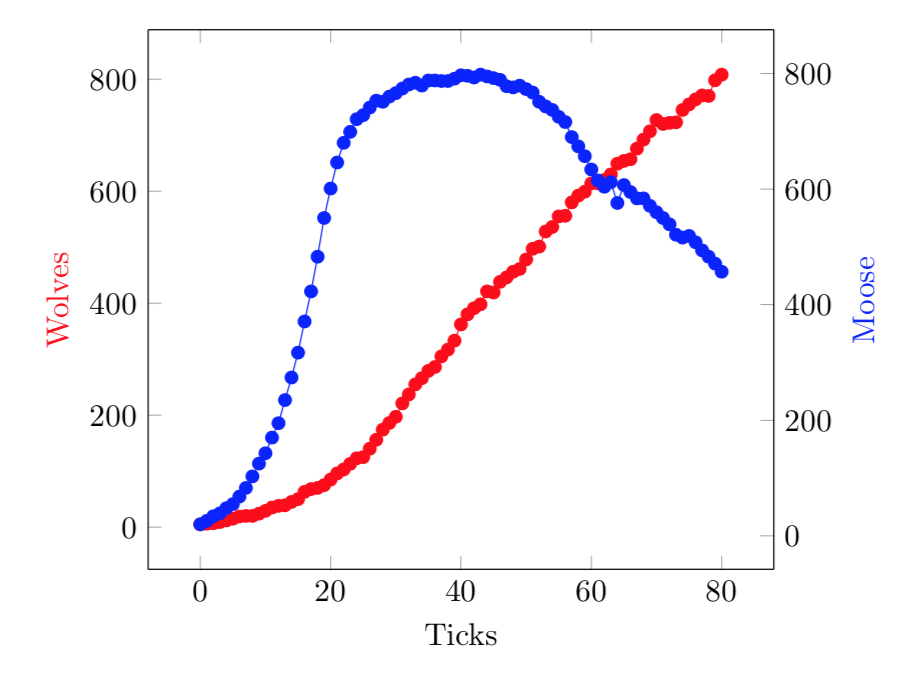
\includegraphics[width=0.60\textwidth]{Experiments/sim_board_b1}
\caption{Input values: ticks: 80, board width: 40, moose: 20, moose rep-length: 5, wolves: 5, wolf rep-lenght: 5, wolf hunger length: 8}
\end{figure}

Figure 2 represent a simulated environment where the board is only 20 X 20. Here, the number of moose becomes approximately 250 at tick 20 while it is 600 at the larger board in Figure 1. The same difference can be observed with the wolves. Another interesting observation is that the moose are extinct at tick 50 - whey get eaten by the wolves in the small amount of space. 

\begin{figure}[H]
\centering
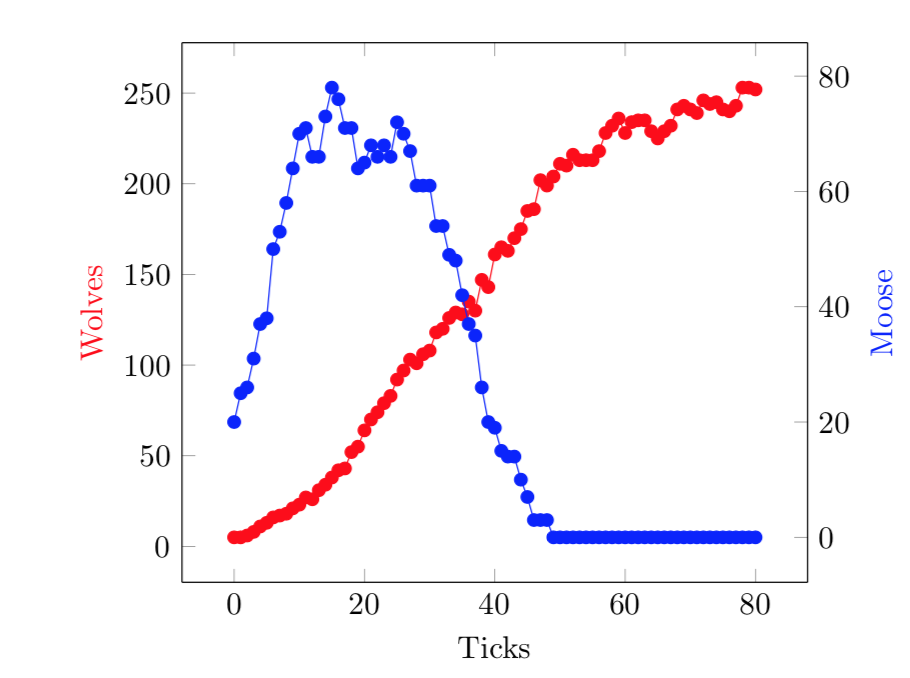
\includegraphics[width=0.60\textwidth]{Experiments/sim_board_b2} 
\caption{Input values: ticks: 80, board width: 20, moose: 20, moose rep-length: 5, wolves: 5, wolf rep-lenght: 5, wolf hunger length: 8}
\end{figure}

\subsubsection*{Hunger length}

Another experiment we have conducted focuses on the hunger length of the wolves. At Figure 3, the hunger length is rather shot, it is set to 4, so after 4 ticks the wolf will either die or have found a moose to eat. The result is, that only after 10 ticks the wolves are extinct while the moose keeps to increase in number.
\begin{figure}[H]
\centering
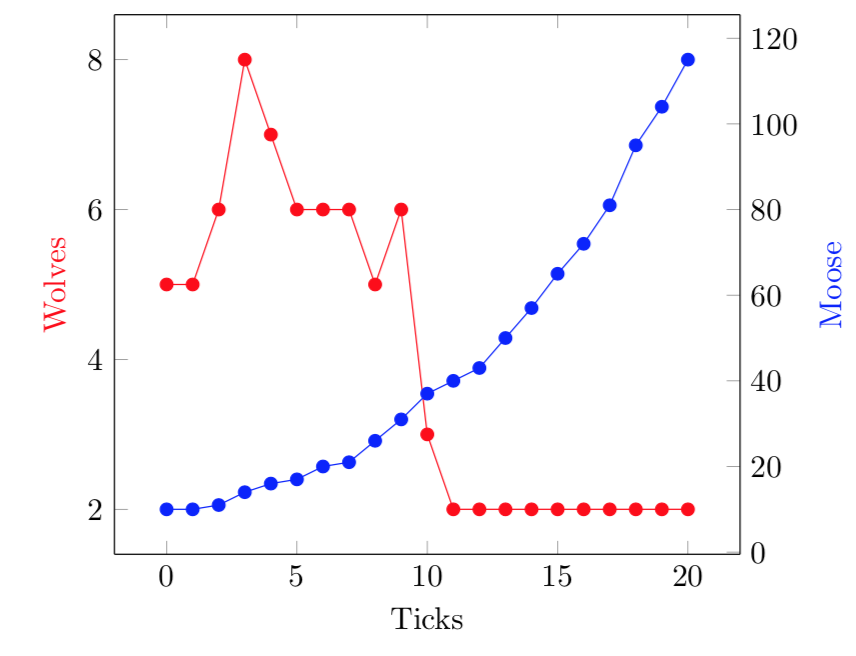
\includegraphics[width=0.60\textwidth]{Experiments/sim_hunlen_a1}
\caption{Input values: ticks: 20, board width: 15, moose: 10, moose rep-length: 5, wolves: 5, wolf rep-length: 5, wolf hunger length: 4}
\end{figure}

When we change the hunger length from 4 to 6 we get another result. As shown in the graph at Figure 4 we see that wolves does not extinct any more, but the moose does instead. At the beginning, the moose increase in number but around tick 10 the amount of wolves are so high that the number of moose start to decrease and at tick 16 they are all dead.

When the hunger length of the wolves is at 6, the wolves can exist for longer without eating. As the reproduction level is smaller than the hunger length, the wolf reproduce itself before it dies, and therefore they cannot extinct in this experiment, even if there are no moose left in the environment. Obviously, this means we should be conscious about the relation between the reproduction and the hunger length.

\begin{figure}[H]
\centering
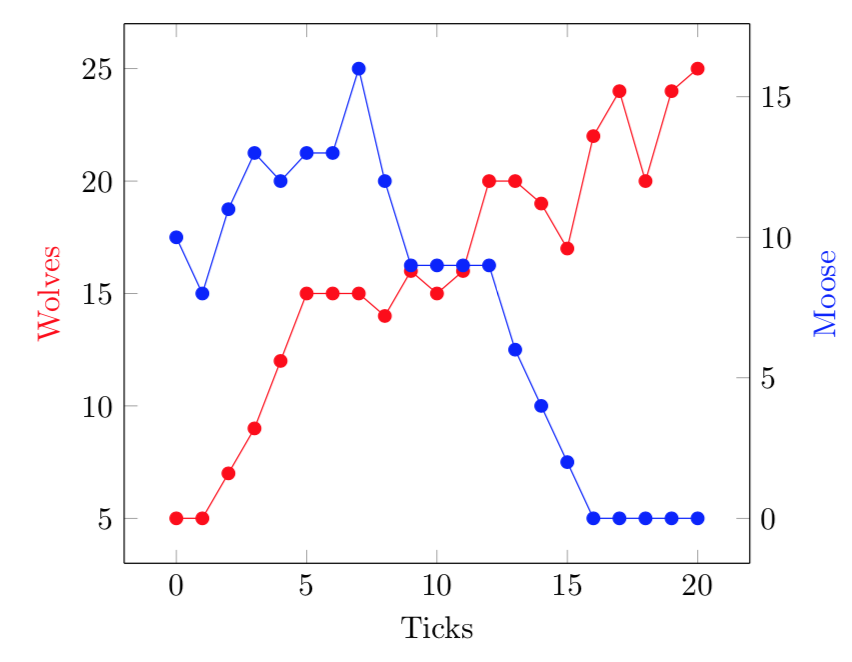
\includegraphics[width=0.60\textwidth]{Experiments/sim_hunlen_a2}
\caption{Input values: ticks: 20, board width: 15, moose: 10, moose reproduction length: 5, wolves: 5, wolf reproduction length: 5, wolf hunger length: 6}
\end{figure}


\subsubsection*{Reproduction length}
At Figure 5 and Figure 6 we see an experiment with variation in reproduction length. At Figure 5, the moose and the wolves have a longer reproduction length than on Figure 6. In both cases the number of moose increase rapidly within the first 20 ticks and then it stagnates.
 
At Figure 5, we clearly see that the number of moose is dependent of the number of wolves and vice versa. At approximately tick 100 the number of moose decrease rapidly while the number of wolves reach 80 - the relation is about 1/5 the amount of moose. Then the number of wolves decreases again when the number of moose has reached a level under 200. The wolves die because of the small amount of food for them. \newline 
Of all of our simulations, this one is probably the one where they can co-exists for the longest time.

\begin{figure}[H]
\centering
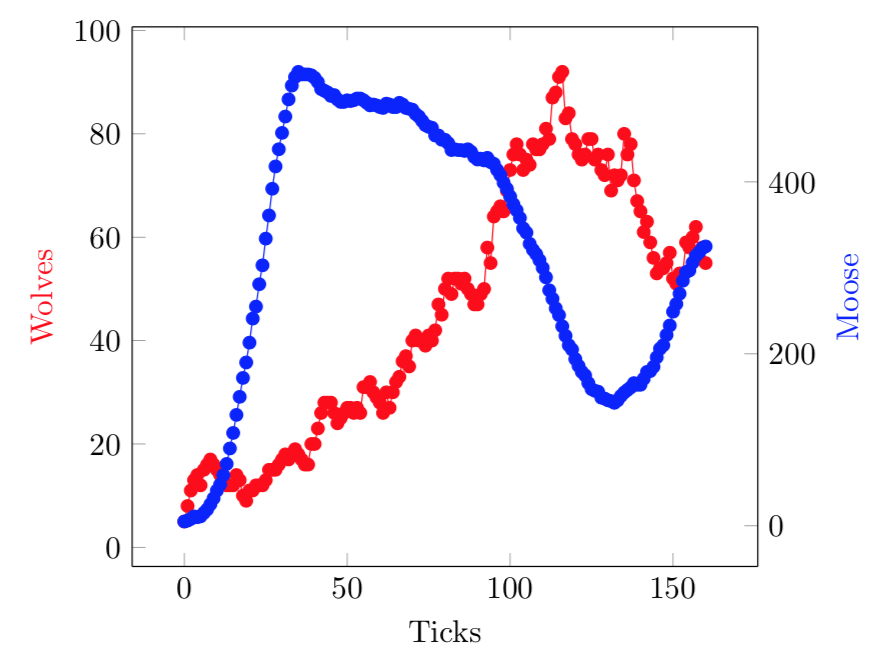
\includegraphics[width=0.60\textwidth]{Experiments/sim_rep_c1}
\caption{Input values: ticks: 150, boardw: 25, moose: 5, moose reproduction length: 4, wolves: 5, wolf reproduction length: 3, wolf hunger length: 4}
\end{figure}

If we change the reproduction length only by one, we see that the number of moose becomes even more, but the opposite can be said for wolves. It takes longer for them to increase significantly, but when they do, again we see that the number of moose decreaces. 


\begin{figure}[H]
\centering
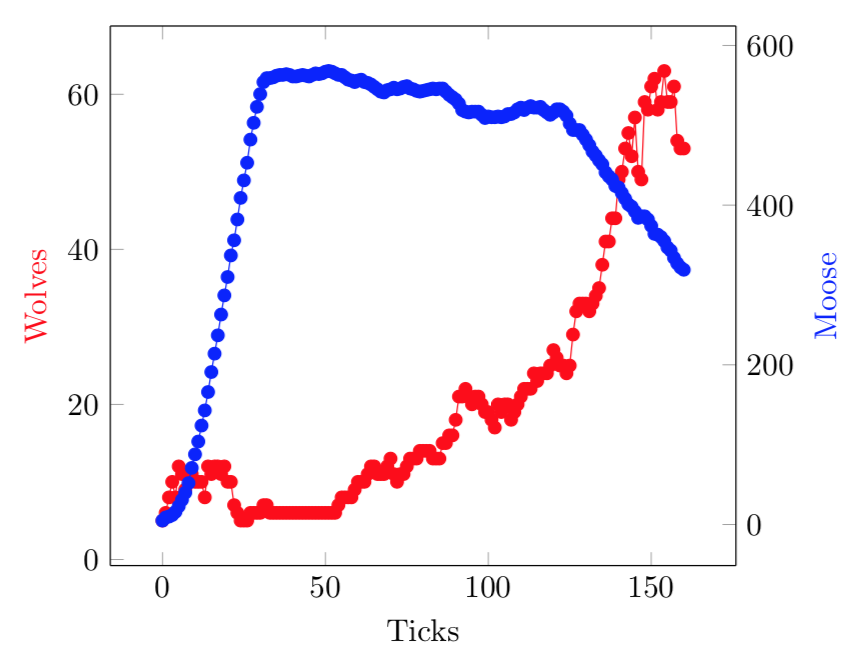
\includegraphics[width=0.60\textwidth]{Experiments/sim_rep_c2}
\caption{Input values: ticks: 160, boardw: 25, mooses: 5, moose rep-lenght: 3, wolves: 5, wolf rep-lenght: 4, wolf hunger lenght: 4}
\end{figure}

\subsection*{Conclusion and discussion}
We solved the problem, and programmed the enviroment to mimic the real world to a certain degree. It is obviously difficult to represent a complicated enviroment with only a handful of parameters, but the representation that we have build is has many similarities to the enviroment. There is a clear correlation between the two poplution of animals.
To improve the representation we could have included the other animals in the enviroment, the seasons, improved the interaction between the wolf and the moose, and considered that the wolf is a social animal. Another aspect that we could have considered would be that of the breeding season and that a moose usually get one calf while the wolf tends to get several cubs.

\newpage
\section*{Appendix}

\subsection*{Brugervejledning - to do}

\subsection*{Programtekst - to do}

\end{document}